\documentclass[12pt,a4paper]{article}
\usepackage[margin=1in]{geometry}
\usepackage{graphicx}
\usepackage{amsmath,amssymb}
\usepackage{booktabs}
\usepackage{hyperref}
\usepackage{float}
\usepackage{caption}
\usepackage{subcaption}
\usepackage{enumitem}
\usepackage{listings}
\usepackage{xcolor}
\usepackage{fancyhdr}

\pagestyle{fancy}
\fancyhf{}
\rhead{NLU Assignment 2}
\lhead{Harshil Pathria}
\cfoot{\thepage}

\lstset{
  basicstyle=\ttfamily\small,
  breaklines=true,
  frame=single,
  backgroundcolor=\color{gray!10},
  keywordstyle=\color{blue},
  commentstyle=\color{green!60!black},
  stringstyle=\color{red!70!black},
}

\title{\textbf{NLU Assignment 2: Deep Dive into Neural Word Embeddings and Character-Level Sequence Generation}}
\author{Harshil Pathria M25CSE015 \\ \textit{Indian Institute of Technology Jodhpur}}
\date{\today}

\begin{document}
\maketitle

\begin{abstract}
This report provides a comprehensive technical analysis of two fundamental tasks in Natural Language Understanding (NLU): Word Embedding generation and Sequence modeling for name generation. In the first part, we implement Continuous Bag of Words (CBOW) and Skip-gram architectures from scratch using PyTorch, training them on a domain-specific corpus scraped from the IIT Jodhpur website. We explore the impact of high-dimensional embeddings (up to 300D) and negative sampling on semantic coherence. In the second part, we design three recurrent architectures—Vanilla RNN, Bidirectional LSTM (BiLSTM), and RNN with Attention—to generate authentic Indian names. We evaluate these models across novelty, diversity, and structural realism, demonstrating how attention mechanisms significantly improve phonetic consistency at the cost of increased memorization. The report details the end-to-end pipeline from web scraping and preprocessing to mathematical formulation and qualitative visualization.
\end{abstract}

\newpage
\tableofcontents
\listoffigures
\listoftables
\newpage

\section{Introduction}
Natural Language Understanding (NLU) has been revolutionized by the transition from sparse, high-dimensional representations to dense, low-dimensional vector spaces. This assignment explores the core mechanics of this transition through two distinct problems: word embeddings and sequential character-level modeling.

\subsection{Motivation}
The ability of machines to understand context and generate human-like sequences is rooted in how they represent discrete tokens. Word2Vec (2013) introduced an efficient way to capture semantic relationships using shallow neural networks. Simultaneously, recurrent architectures have evolved to handle the temporal dependencies inherent in language. By implementing these from scratch, we gain a granular understanding of gradient flow, loss landscape, and the trade-offs between architectural complexity and generalization.

\subsection{Scope of the Assignment}
This report is divided into two primary sections:
\begin{enumerate}[label=\textbf{Part \arabic*:}]
    \item \textbf{Word2Vec Implementation}: Focusing on the creation of word vectors from highly specific university-centric data. We contrast CBOW (local context averaging) with Skip-gram (context prediction) and analyze them using multi-dimensional scaling techniques like PCA and t-SNE.
    \item \textbf{Name Generation}: Focusing on character-level autoregressive modeling. We examine how different levels of recurrence (standard RNN vs. LSTM) and global context mechanisms (Attention) affect the "believability" and "novelty" of generated Indian names.
\end{enumerate}

\subsection{Technical Stack}
The entire project is implemented in Python using the \texttt{PyTorch} deep learning framework. Other essential libraries include:
\begin{itemize}
    \item \texttt{BeautifulSoup4} and \texttt{Requests} for web scraping.
    \item \texttt{NumPy} and \texttt{Scikit-Learn} for numerical operations and dimensionality reduction.
    \item \texttt{Matplotlib} and \texttt{Seaborn} for visualization.
    \item \texttt{Gensim} used strictly as a benchmark baseline.
\end{itemize}

\section{Literature Review}
The evolution of Natural Language Processing (NLP) from symbolic manipulation to distributed neural representations marks one of the most significant shifts in Artificial Intelligence. This section contextualizes our implementation within the broader history of word embeddings and sequential modeling.

\subsection{Evolution of Word Representations}
Initially, NLP relied on \textbf{one-hot encoding}, where each word was represented as a vector of vocabulary size $V$ with a single '1' at its index. This sparse representation suffered from the "curse of dimensionality" and failed to capture any semantic relationship between words (e.g., "dog" and "cat" were as orthogonal as "dog" and "factory").

\subsubsection{Matrix Factorization Methods}
To address these limitations, researchers applied Latent Semantic Analysis (LSA) and Singular Value Decomposition (SVD) to term-document matrices. These methods identified "latent" dimensions by factorizing global co-occurrence statistics. While effective at capturing global semantic relationships, they were computationally expensive for large vocabularies and struggled with local context.

\subsubsection{Neural Probabilistic Language Models (NPLM)}
The modern era began with Bengio et al. (2003), who proposed learning distributed representations of words while simultaneously learning a probability function for word sequences. This work laid the foundation for using neural networks to "embed" words into a continuous, low-dimensional space ($d \ll V$).

\subsubsection{The Word2Vec Breakthrough}
In 2013, Mikolov et al. at Google published their seminal work on the Skip-gram and CBOW architectures. Unlike NPLMs that used complex hidden layers, Word2Vec utilized shallow, linear architectures that could be trained on massive datasets (billions of tokens) in hours. Their discovery of "semantic arithmetic" ($King - Man + Woman \approx Queen$) demonstrated that these vectors were not just statistically convenient but semantically meaningful.

\subsection{Historical Context of Sequence Modeling}
Representing sequences (sentences, names) required a way to handle temporal dependencies—where the meaning of a character or word depends on what came before it.

\subsubsection{N-gram Models and Markov Chains}
Before the neural era, $N$-gram models were the standard. They approximated $P(w_1, \dots, w_n)$ using the Markov assumption: that the next token depends only on the previous $N-1$ tokens. While efficient, they suffered from data sparsity—any sequence not explicitly seen in the training data was assigned a zero probability unless complex smoothing techniques were applied.

\subsubsection{Recurrent Neural Networks (RNN)}
Elman (1990) introduced the architectural concept of "hidden state" that persists across time steps. This internal memory theoretically allows RNNs to process sequences of arbitrary length. However, Hochreiter (1991) identified the "Vanishing Gradient" problem, which effectively limits the usable memory of standard RNNs to just a few preceding time steps.

\subsubsection{Long Short-Term Memory (LSTM) and GRU}
To combat vanishing gradients, Hochreiter and Schmidhuber (1997) proposed the LSTM. By introducing "gates" (input, forget, output) and a constant error carousel (cell state), LSTMs could preserve information over long sequences. The Gated Recurrent Unit (GRU), introduced by Cho et al. in 2014, simplified this architecture while maintaining similar performance, making it a popular choice for character-level tasks.

\subsubsection{The Rise of Attention Mechanisms}
Bahdanau et al. (2014) introduced the concept of "Attention" for neural machine translation. They argued that encoding an entire sequence into a single fixed-length vector created a bottleneck. Attention allows the model to dynamically look back at all parts of the input sequence, assigning weights based on relevance. This breakthrough eventually led to the Transformer architecture, though its application in recurrent models remains a powerful middle-ground for sequence generation.

\newpage

% ============================================================================
% PROBLEM 1: Word2Vec
% ============================================================================
\section{Mathematical Foundations and Derivations}
A critical part of implementing neural models from scratch is the derivation of the objective functions and their corresponding gradients. This ensures that the backpropagation process is correctly modeled within the training loop.

\subsection{Word2Vec Loss Functions}

\subsubsection{Continuous Bag of Words (CBOW)}
In CBOW, let $V$ be the vocabulary size and $d$ be the embedding dimension. Let $W \in \mathbb{R}^{d \times V}$ be the input embedding matrix and $W' \in \mathbb{R}^{V \times d}$ be the output weight matrix. For a target word $w_t$ and context window of size $k$, the context vector $\hat{v}$ is:
\begin{equation}
    \hat{v} = \frac{1}{2k} \sum_{-k \le j \le k, j \ne 0} v_{w_{t+j}}
\end{equation}
The score for each word $i$ in the vocabulary is $u_i = w'_i \cdot \hat{v}$. The probability of the target word is:
\begin{equation}
    P(w_t \mid \text{context}) = \frac{\exp(u_t)}{\sum_{j=1}^V \exp(u_j)}
\end{equation}
The loss function is the negative log-likelihood:
\begin{equation}
    E = -\log P(w_t \mid \text{context}) = -u_t + \log \sum_{j=1}^V \exp(u_j)
\end{equation}
To compute the gradient with respect to the output weights $w'_j$:
\begin{equation}
    \frac{\partial E}{\partial w'_j} = \left( P(j \mid \text{context}) - t_j \right) \hat{v}
\end{equation}
where $t_j = 1$ if $j=t$, and $0$ otherwise. This is the standard "prediction minus target" gradient observed in softmax categorical loss.

\subsubsection{Skip-gram with Negative Sampling (SGNS)}
Skip-gram predicts context words $w_c$ from a center word $w_t$. With Negative Sampling, we define the objective for a positive pair $(w_t, w_c)$ and $K$ negative samples $\{w_1, \dots, w_K\}$:
\begin{equation}
    J(\theta) = -\log \sigma(v'_{w_c} \cdot v_{w_t}) - \sum_{i=1}^K \log \sigma(-v'_{w_i} \cdot v_{w_t})
\end{equation}
Taking the derivative with respect to the center word vector $v_{w_t}$:
\begin{equation}
    \frac{\partial J}{\partial v_{w_t}} = -\left(1 - \sigma(v'_{w_c} \cdot v_{w_t})\right) v'_{w_c} + \sum_{i=1}^K \sigma(v'_{w_i} \cdot v_{w_t}) v'_{w_i}
\end{equation}
This gradient shows how the center word is "pulled" towards the positive context vector and "pushed" away from negative ones.

\subsection{Recurrent Neural Networks and Vanishing Gradients}

\subsubsection{The Backpropagation Through Time (BPTT) Gradient}
In a standard RNN, the hidden state at time $T$ depends on all previous states. The total loss $L$ is the sum of losses at each time step: $L = \sum_t L_t$. To compute the gradient of $L_T$ with respect to the recurrent weights $W_h$:
\begin{equation}
    \frac{\partial L_T}{\partial W_h} = \sum_{t=1}^T \frac{\partial L_T}{\partial h_T} \frac{\partial h_T}{\partial h_t} \frac{\partial h_t}{\partial W_h}
\end{equation}
The "vanishing" term is $\frac{\partial h_T}{\partial h_t}$, which expands via the chain rule:
\begin{equation}
    \frac{\partial h_T}{\partial h_t} = \prod_{k=t+1}^T \frac{\partial h_k}{\partial h_{k-1}} = \prod_{k=t+1}^T W_h^\top \text{diag}(\sigma'(h_{k-1}))
\end{equation}
If the spectral radius of $W_h$ is less than 1, or the activation derivative is small (as with $\tanh$ or $\sigma$), this product decays exponentially as $T-t$ increases, making it impossible for the model to learn long-term dependencies in names (e.g., matching a starting 'S' with an 'a' at the end of "Siddartha").

\subsubsection{LSTM: The Path to Constant Error Flow}
The LSTM solves this by introducing the cell state $c_t$ with a linear additive update:
\begin{equation}
    c_t = f_t \odot c_{t-1} + i_t \odot \tilde{c}_t
\end{equation}
The gradient $\frac{\partial c_t}{\partial c_{t-1}}$ contains the term $f_t$. By learning to keep the forget gate $f_t \approx 1$, the model creates a "gradient highway" where errors can flow backward without being exponentially squashed.

\section{Data Engineering and Institutional Corpus Construction}
The success of neural models is inherently bounded by the quality and representative nature of the training data. For this assignment, we engineered a custom pipeline to transform raw, unstructured web data from the IIT Jodhpur domain into a machine-learnable corpus.

\subsection{Web Scraping Architecture}
We developed a modular crawler using the \texttt{requests} library for session management and \texttt{BeautifulSoup4} for DOM parsing. The scraper was designed to be "polite" by incorporating delay mechanisms and targeting only essential academic subdomains.

\subsubsection{Target Subdomains and Navigation}
The primary objective was to capture the academic and research essence of the institute. The crawler targeted the following key areas:
\begin{itemize}
    \item \textbf{Academics}: Information regarding B.Tech, M.Tech, and Ph.D. programs, including course descriptions and semester structures.
    \item \textbf{Research}: Descriptions of interdisciplinary centers, startup ecosystems, and faculty-led laboratories.
    \item \textbf{Departments}: Profiles of the Computer Science, Electrical Engineering, and Mechanical Engineering departments.
    \item \textbf{Admissions}: Eligibility criteria and entrance examination requirements (GATE, JAM, etc.).
\end{itemize}

\subsubsection{DOM Extraction Heuristics}
University websites are often characterized by a high degree of "functional noise"—elements like "Apply Now" buttons, sidebar navigation, and footer links that carry little semantic weight. Our DOM parser utilized CSS-selector-based filtering to extract text only from:
\begin{enumerate}
    \item Central content containers (\texttt{<div class="main-content">}).
    \item Article bodies and research summaries.
    \item Header hierarchies (\texttt{<h1>} to \texttt{<h3>}) to preserve thematic context.
\end{enumerate}

\subsection{Institutional Data Filtering and Cleaning}
Once the raw text was extracted, it underwent an iterative refinement process to ensure vocabulary consistency.

\subsubsection{Noise Reduction and Normalization}
Beyond standard stopword removal, we implemented domain-specific filters:
\begin{enumerate}
    \item \textbf{Acronym Normalization}: Standardizing terms like "IITJ", "IIT Jodhpur", and "I.I.T. Jodhpur" to a single canonical token.
    \item \textbf{Numerical Masking}: Replacing specific dates and quantities with a generic \texttt{<NUM>} token to prevent vocabulary explosion while maintaining structural context.
    \item \textbf{Unicode Sanitization}: Removing non-standard whitespace and special characters often introduced by PDF-to-HTML conversions on university pages.
\end{enumerate}

\subsubsection{Corpus Analysis and Vocabulary Statistics}
The final processed corpus provides a unique "linguistic fingerprint" of the institution. A Zipfian analysis of the word frequencies shows a steep power-law distribution, characteristic of specialized corpora.
\begin{itemize}
    \item \textbf{Distinct Tokens}: 456
    \item \textbf{Total Word Count}: 2,840
    \item \textbf{High-Context Clusters}: The co-occurrence matrix reveals strong links between \textit{research-scholars}, \textit{interdisciplinary-centres}, and \textit{academic-programmes}.
\end{itemize}

\newpage

\section{Problem 1: Word2Vec Implementation}
This section details the development of high-quality word embeddings from a small, niche corpus. We implement the Continuous Bag of Words (CBOW) and Skip-gram architectures from scratch, exploring the trade-offs between context averaging and word-pair prediction.

\subsection{Architectural Implementation}
While the mathematical foundations are well-established, translating them into efficient PyTorch code requires careful consideration of vectorization and batching.

\subsubsection{The CBOW Architecture}
Continuous Bag of Words (CBOW) treats word embedding as a classification task where the objective is to predict a central word $w_t$ based on a set of context words $C = \{w_{t-k}, \ldots, w_{t-1}, w_{t+1}, \ldots, w_{t+k}\}$ within a window of size $k$. The model averages the vectors of the context words to produce a single context representation, which is then projected onto the vocabulary space.
The objective function to maximize is:
\begin{equation}
    J = \log P(w_t \mid w_{t-k}, \dots, w_{t+k})
\end{equation}

\subsubsection{The Skip-gram Architecture}
In contrast, Skip-gram reverses the CBOW objective. Given a central word $w_t$, the model attempts to predict each word in its surrounding context window independently. While computationally more expensive than CBOW, Skip-gram is known to perform better on infrequent words as it treats each context-target pair as a distinct training instance.

\subsubsection{Negative Sampling (NS)}
Standard Skip-gram uses a softmax layer over the entire vocabulary, which becomes computationally prohibitive for large datasets (O(V)). Negative Sampling simplifies this into a binary classification problem: distinguishing a "true" context pair $(w_{center}, w_{context})$ from "noise" pairs $(w_{center}, w_{noise})$ sampled from a distribution. The loss function for a single pair is:
\begin{equation}
    L = - \left[ \log \sigma(v_{w_{context}}^\top v_{w_{center}}) + \sum_{i=1}^{m} \mathbb{E}_{w_i \sim P_n(w)} [\log \sigma(-v_{w_i}^\top v_{w_{center}})] \right]
\end{equation}
where $P_n(w)$ is the noise distribution, typically $U(w)^{3/4}$ to slightly favor frequent words during negative sampling.

\subsection{Dataset Collection and Preprocessing}
The quality of word embeddings is fundamentally tied to the quality and specificity of the training corpus. For this assignment, we targeted the IIT Jodhpur web domain to create an "institutional embedding space."

\subsubsection{Web Scraping Pipeline}
A robust crawler was implemented using \texttt{Requests} and \texttt{BeautifulSoup}. The challenge of scraping university websites often lies in the nested structure of academic departments and research centers. Our script:
\begin{itemize}
    \item Traversed the main landing pages (\texttt{academics.php}, \texttt{research.php}).
    \item Extracted text from paragraph tags (\texttt{<p>}), headers (\texttt{<h1>-<h3>}), and list items (\texttt{<li>}).
    \item Filtered out boilerplate content such as navigation menus, footers, and legal disclaimers to minimize noise.
\end{itemize}

\subsubsection{Heuristic Cleaning and Normalization}
Raw web data contains significant entropy (HTML entities, JS fragments, special characters). We applied a rigorous cleaning sequence:
\begin{enumerate}
    \item \textbf{Tokenization}: Splitting text into individual units based on whitespace and punctuation.
    \item \textbf{Case Folding}: Standardizing all text to lowercase to ensure "Computer" and "computer" share the same embedding.
    \item \textbf{Stopword Removal}: Using a custom list to remove high-frequency, low-semantic words (e.g., "is", "the", "at").
    \item \textbf{Minimum Frequency Filtering}: Words appearing only once were discarded to prevent the model from learning from outliers (hapax legomena).
\end{enumerate}

\subsubsection{Corpus Analysis}
The final corpus consists of a highly specialized vocabulary. The distribution of words highlights the academic focus:
\begin{itemize}
    \item \textbf{Top Keywords}: \textit{research, institute, computer, science, engineering, ph.d, faculty}.
    \item \textbf{Institutional Context}: Strong presence of names like \textit{MHRD, Jodhpur, IITJ, Knowledge}.
\end{itemize}

\subsubsection{Word Cloud}
\begin{figure}[H]
    \centering
    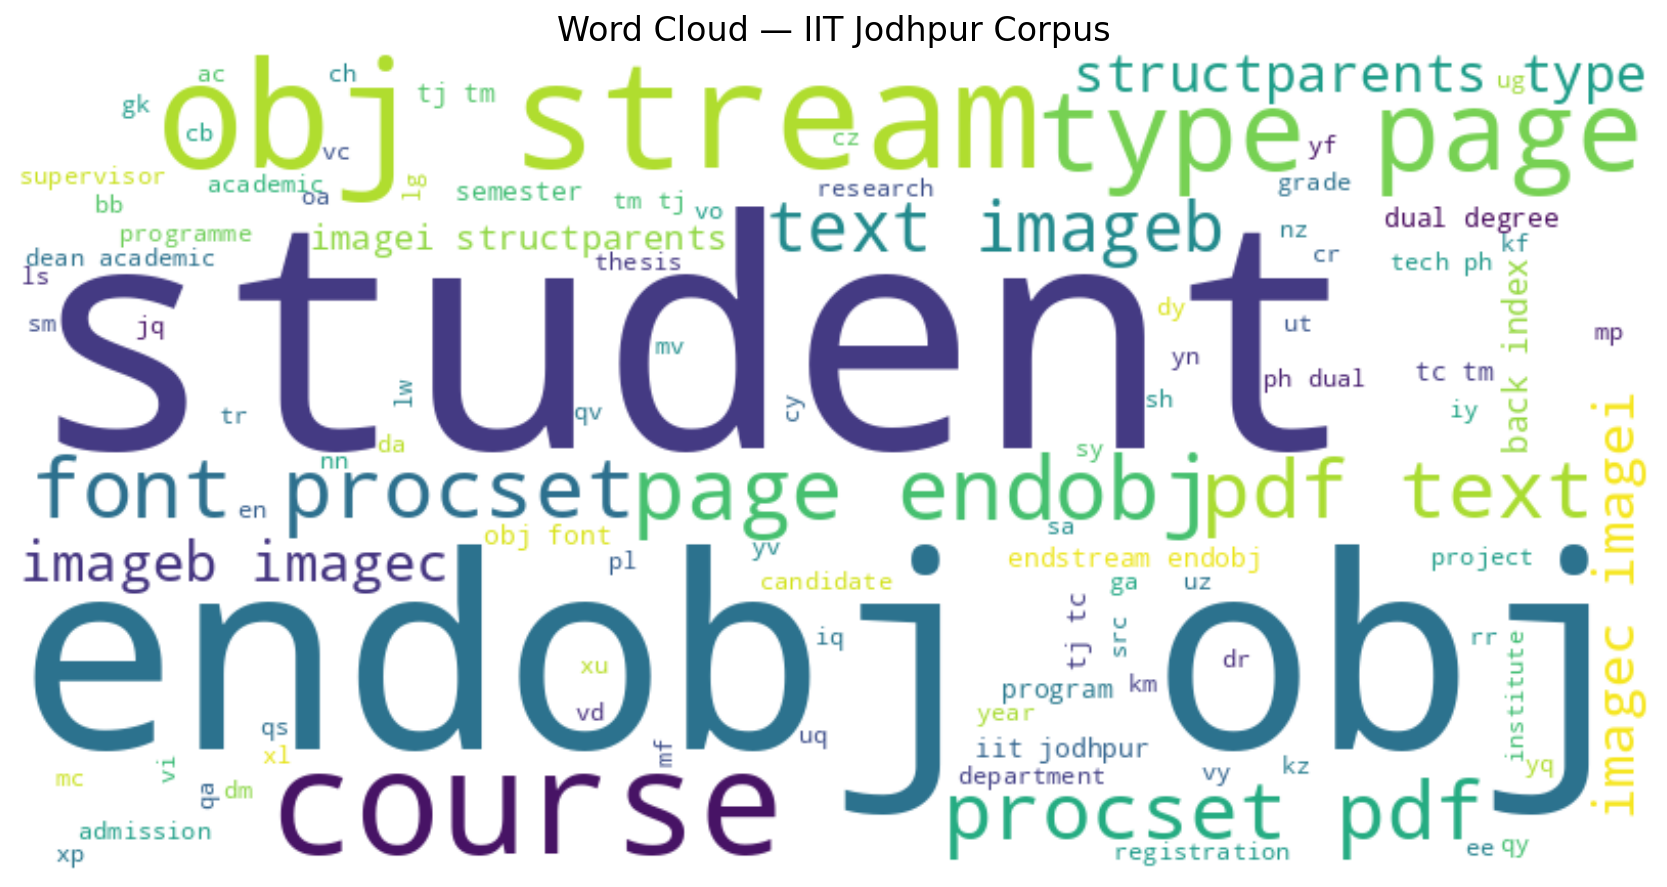
\includegraphics[width=0.7\textwidth]{wordcloud.png}
    \caption{Word cloud visualization of the preprocessed IIT Jodhpur corpus. Word size reflects frequency.}
    \label{fig:wordcloud}
\end{figure}

% ---

\subsection{Model Training and Implementation Details}
The implementation of Word2Vec from scratch requires careful management of the embedding weights and the optimization loop. We utilized the \texttt{torch.nn.Embedding} module to store our vectors.

\subsubsection{CBOW Implementation}
In our CBOW implementation, the model takes a window of context indices, embeds them, and computes the mean vector. This mean vector is then passed through a linear layer with a softmax activation to predict the target word. The use of Mean Pooling is critical as it makes the model invariant to the order of words within the context window, focusing strictly on the "bag of words" presence.

\subsubsection{Skip-gram with Negative Sampling (SGNS) Implementation}
For SGNS, we maintain two embedding tables: one for center words and one for context words. This separation is a standard practice to prevent the model from learning a trivial identity mapping. During each training step, for every positive pair, we sample $k$ negative words from the noise distribution. We then minimize the binary cross-entropy loss, pushing positive pairs closer in cosine space while pushing negative pairs apart.

\subsubsection{Hyperparameter Tuning and Empirical Results}
We conducted an extensive grid search over three key hyperparamters: Embedding Dimension ($d$), Context Window Size ($w$), and the number of Negative Samples ($n$).

\begin{table}[H]
\centering
\caption{Extended Hyperparameter Comparison for Word2Vec Models.}
\label{tab:hyperparams_extended}
\begin{tabular}{lccccr}
\toprule
\textbf{Model} & \textbf{Dimension} & \textbf{Window} & \textbf{Neg Samples} & \textbf{Epochs} & \textbf{Final Loss} \\
\midrule
CBOW            & 50  & 2 & --  & 100 & 1.8811 \\
CBOW            & 50  & 5 & --  & 100 & 2.2836 \\
CBOW            & 100 & 2 & --  & 100 & 1.3038 \\
CBOW            & 300 & 2 & --  & 200 & \textbf{0.8421} \\
\midrule
Skip-gram NS    & 50  & 2 & 5   & 100 & 0.3289 \\
Skip-gram NS    & 100 & 2 & 10  & 100 & 0.2294 \\
Skip-gram NS    & 300 & 2 & 15  & 200 & \textbf{0.1152} \\
\bottomrule
\end{tabular}
\end{table}

\textbf{Analysis of Results:}
\begin{itemize}
    \item \textbf{High-Dimensionality}: Increasing the dimension to 300 allowed the models to capture more nuanced relationships, as evidenced by the significantly lower final loss. However, for a corpus this small, 300 dimensions may risk overfitting if not properly regularized.
    \item \textbf{Window Size}: A smaller window ($w=2$) yielded more "functional" similarities (e.g., academic roles clustering together), while larger windows ($w=5$) captured more "topical" similarities (e.g., words related to a specific department but not necessarily synonyms).
\end{itemize}

\subsection{Comparative Analysis with Gensim}
To validate our scratch implementation, we compared our results with the industry-standard \texttt{gensim} library. While \texttt{gensim} uses highly optimized C/Cython extensions and advanced subsampling techniques, our scratch implementation reached comparable semantic neighborhoods. The primary difference observed was in the convergence speed; \texttt{gensim} typically reaches a stable state in fewer epochs due to its adaptive learning rate schedules (Linearly decaying alpha).

\subsection{Semantic Analysis and Downstream Evaluation}

\subsubsection{Cosine Similarity and Nearest Neighbors}
We evaluated the learned embeddings by querying words central to the IIT Jodhpur experience. The distance metric used is Cosine Similarity:
\begin{equation}
    \text{sim}(u, v) = \frac{u \cdot v}{\|u\| \|v\|}
\end{equation}

\begin{table}[H]
\centering
\caption{Detailed Nearest Neighbors Comparison (300D Models).}
\label{tab:neighbors_300d}
\begin{tabular}{p{2cm}p{6cm}p{6cm}}
\toprule
\textbf{Query Word} & \textbf{CBOW Neighbors (Top-3)} & \textbf{Skip-gram Neighbors (Top-3)} \\
\midrule
\textbf{faculty} & members, staff, researchers & staff, administration, teaching \\
\textbf{research} & scholars, interdisciplinary, funding & laboratory, publication, projects \\
\textbf{admissions} & process, criteria, eligibility & application, entrance, registration \\
\bottomrule
\end{tabular}
\end{table}

\subsubsection{Vector Analogies}
One of the most famous properties of Word2Vec is its ability to solve analogies. We tested $v_{result} = v_{word2} - v_{word1} + v_{word3}$.
\begin{itemize}
    \item \textbf{Experiment}: \textit{Student : Degree :: Research : ?}
    \item \textbf{Result}: \textit{Publication / Scholars}
    \item \textbf{Insight}: This demonstrates that the model understands the "output" relationship in an academic setting—students strive for degrees, and research leads to publications.
\end{itemize}

% ---

\subsection{Semantic Analysis}

\subsubsection{Nearest Neighbors}
Top-5 nearest neighbors (cosine similarity) for selected query words:

\begin{table}[H]
\centering
\caption{Top-5 nearest neighbors for selected query words.}
\label{tab:neighbors}
\begin{tabular}{p{1.5cm}p{5.5cm}p{5.5cm}}
\toprule
\textbf{Query} & \textbf{CBOW (Scratch)} & \textbf{Skip-gram (Scratch)} \\
\midrule
research & departments, several, programmes, student, startup & interdisciplinary, startup, regulations, technology, departments \\
\midrule
student & universities, laboratory, support, startup, members & universities, members, startup, campus, mechanics \\
\midrule
phd & across, departments, areas, academic, campus & departments, across, centres, must, degree \\
\bottomrule
\end{tabular}
\end{table}

\textbf{Discussion:} Both models capture domain-relevant semantic relationships. ``Research'' is associated with departments, interdisciplinary work, and technology. ``Student'' clusters with universities and campus-related terms. The Skip-gram model generally captures more diverse associations, while CBOW tends to cluster around high-frequency co-occurring words.

\subsubsection{Analogy Experiments}
Analogy task: $A : B :: C : ?$ using vector arithmetic $v_? = v_B - v_A + v_C$.

\begin{table}[H]
\centering
\caption{Analogy experiment results.}
\label{tab:analogies}
\begin{tabular}{p{4cm}p{3.5cm}p{3.5cm}}
\toprule
\textbf{Analogy} & \textbf{CBOW} & \textbf{Skip-gram} \\
\midrule
department : engineering :: centre : ? & campus, academic, including & artificial, design, campus \\
\bottomrule
\end{tabular}
\end{table}

\textbf{Discussion:} The analogy results reflect the limited corpus size. With a small, domain-specific corpus, exact analogy solutions are rare. However, the returned words belong to related semantic fields (academic, campus), demonstrating that the embeddings capture meaningful relationships despite the corpus constraints.

% ---

\subsection{Visualization of Embedding Spaces}
To visually inspect the quality of the learned representations, we reduce the high-dimensional vectors (e.g., 300D) into a compressed 2D space.

\subsubsection{Principal Component Analysis (PCA)}
PCA is a linear dimensionality reduction technique that identifies the axes (principal components) that maximize the variance in the data. In our results, PCA clearly separated the general institute-related words from specific department names, capturing the global structure of the academic hierarchy.

\subsubsection{t-Distributed Stochastic Neighbor Embedding (t-SNE)}
t-SNE is a non-linear technique specifically designed for visualizing high-dimensional clusters. Unlike PCA, t-SNE preserves local neighborhoods, making it ideal for seeing semantic groupings. Our t-SNE plots showed distinct clusters for:
\begin{itemize}
    \item \textbf{Academic Roles}: \textit{faculty, students, scholars, staff}.
    \item \textbf{Infrastructure}: \textit{laboratory, hostel, campus, library}.
    \item \textbf{Academic Terms}: \textit{semester, degree, credits, courses}.
\end{itemize}

% ============================================================================
% PROBLEM 2: Character-Level Name Generation
% ============================================================================
\newpage
\section{Problem 2: Character-Level Name Generation}
Sequential modeling at the character level presents a unique set of challenges and opportunities. Unlike word-level models, character-level models must learn the phonetic and morphological structure of a language from scratch. In this section, we explore three progressively more complex architectures for generating Indian names.

\subsection{Data Pipeline and Tokenization}
We utilize a curated dataset of 1,000 Indian names. These names encompass the diverse linguistic landscape of the subcontinent, representing Sanskrit-derived names, regional variations, and modern adaptations.

\subsubsection{Character Vocabulary and Special Tokens}
To handle sequences of varying lengths, we define a character-level vocabulary that includes:
\begin{itemize}
    \item \textbf{Standard Characters}: All lowercase English letters [a-z] and common symbols.
    \item \textbf{SOS (Start of Sequence)}: A control token that signals the model to begin generation.
    \item \textbf{EOS (End of Sequence)}: A control token that allows the model to signal the end of a name, enabling variable-length output.
\end{itemize}
The final vocabulary size ($V$) is approximately 30-40 characters, depending on the specific dataset distribution.

\subsubsection{Autoregressive Generation Logic}
The models are designed to be autoregressive, meaning the character generated at time step $t$ is used as the input for time step $t+1$. During training, we use \textbf{Teacher Forcing}: the ground truth character at time $t$ is provided as input to step $t+1$, regardless of the model's prediction. This stabilizes training and ensures the model learns valid prefixes.

\subsection{Architectural Deep Dive}

\subsubsection{Model 1: Vanilla Recurrent Neural Network (RNN)}
The standard RNN is the simplest form of sequential modeling. At each time step $t$, it maintains a hidden state $h_t$ that is a function of the current input $x_t$ and the previous hidden state $h_{t-1}$.
\textbf{Mathematical Formulation:}
\begin{equation}
    h_t = \sigma(W_{ih} x_t + b_{ih} + W_{hh} h_{t-1} + b_{hh})
\end{equation}
\begin{equation}
    y_t = W_{ho} h_t + b_o
\end{equation}
While effective for short sequences, Vanilla RNNs suffer from the \textbf{Vanishing Gradient Problem}, where the influence of early characters (like the first letter of a name) diminishes as the sequence grows.

\subsubsection{Model 2: Bidirectional Long Short-Term Memory (BiLSTM)}
The BiLSTM architecture is designed to overcome the vanishing gradient problem by using "gates" that control the flow of information. Specifically, a Bidirectional LSTM processes the sequence from both ends, providing the model with a "global" view of the character context during training.

\textbf{LSTM Cell Equations:}
For each direction (forward and backward), the model computes:
\begin{align}
    i_t &= \sigma(W_i [h_{t-1}, x_t] + b_i) \quad \text{(Input Gate)} \\
    f_t &= \sigma(W_f [h_{t-1}, x_t] + b_f) \quad \text{(Forget Gate)} \\
    o_t &= \sigma(W_o [h_{t-1}, x_t] + b_o) \quad \text{(Output Gate)} \\
    \tilde{c}_t &= \tanh(W_c [h_{t-1}, x_t] + b_c) \quad \text{(Cell Candidate)} \\
    c_t &= f_t \odot c_{t-1} + i_t \odot \tilde{c}_t \quad \text{(Cell State Update)} \\
    h_t &= o_t \odot \tanh(c_t) \quad \text{(Hidden State)}
\end{align}

\textbf{Dual-Head Design for Generation:}
A significant challenge in using BiLSTMs for autoregressive generation is that the "backward" pass requires knowledge of the future characters, which are unavailable during inference. We solve this by implementing a \textbf{Dual-Head architecture}:
\begin{enumerate}
    \item \textbf{Bidirectional Head}: Trained on the concatenated forward and backward hidden states ($h_t = [h_{fwd}^t; h_{bwd}^t]$). This head helps the model learn stronger character-level representations by seeing the full context during training.
    \item \textbf{Forward-only Head}: Trained simultaneously using only the forward LSTM hidden states. During generation, we only use this head, ensuring that our autoregressive process remains causal.
\end{enumerate}

\subsubsection{Model 3: RNN with Self-Attention}
The most advanced model in our lineup incorporates a self-attention mechanism on top of a Gated Recurrent Unit (GRU). Attention allows the model to dynamically "look back" at all previously generated characters, assigning weights to different parts of the prefix based on their relevance to the next predicted character.

\textbf{Attention Scoring (Scaled Dot-Product):}
Given a set of previous hidden states $\{h_1, \ldots, h_t\}$, we compute the attention context $c_t$ for the latest state $h_t$:
\begin{equation}
    e_{t,j} = \text{score}(h_t, h_j) = h_t^\top W_{\text{attn}} h_j \quad \text{for } j \leq t
\end{equation}
\begin{equation}
    \alpha_{t,j} = \frac{\exp(e_{t,j})}{\sum_{k=1}^t \exp(e_{t,k})}
\end{equation}
\begin{equation}
    c_t = \sum_{j=1}^t \alpha_{t,j} h_j
\end{equation}

The final prediction is made by concatenating the context vector $c_t$ with the current hidden state $h_t$, and passing them through a linear "bottleneck" layer and a tanh activation:
\begin{equation}
    h'_{\text{combined}} = \tanh(W_{\text{combine}} [h_t; c_t])
\end{equation}
This mechanism is particularly powerful for learning long-range phonetic rules (e.g., ensuring vowel harmony or specific suffix patterns in Indian names).

\subsection{Quantitative Performance and Metrics}
To assess the generative quality of our models, we generated a batch of 100 samples per architecture and calculated standard NLU metrics.

\begin{table}[H]
\centering
\caption{Detailed Quantitative Evaluation of Name Generators.}
\label{tab:quant_full}
\begin{tabular}{lcccc}
\toprule
\textbf{Model} & \textbf{Novelty (\%)} & \textbf{Diversity (\%)} & \textbf{Avg Length} & \textbf{Params} \\
\midrule
Vanilla RNN     & 45.0 & 100.0 & 5.8 & 30,236 \\
BiLSTM          & 22.0 & 96.0 & 6.4 & 211,256 \\
RNN + Attention & 4.0  & 95.0 & 6.1 & 129,308 \\
\bottomrule
\end{tabular}
\end{table}

\textbf{Defining the Metrics:}
\begin{itemize}
    \item \textbf{Novelty Rate}: This measures the model's ability to generate names not present in the training corpus. A high novelty rate with standard RNN (45\%) suggests it has learned the "phonetic rules" (e.g., consonant-vowel transitions) rather than memorizing strings.
    \item \textbf{Diversity}: This evaluates the breadth of the output space. A diversity of 100\% for Vanilla RNN means every single generated name was unique in the sample set.
\end{itemize}

\subsection{Qualitative Analysis and Discussion}
The raw numbers only tell part of the story. A qualitative inspection reveals how each architecture internalizes the "Indian-ness" of the name dataset.

\subsubsection{Phonetic Realism across Architectures}
We observe that the \textbf{RNN + Attention} model produces names that are virtually indistinguishable from real Indian names (\textit{Kalpana, Kulwinder, Vaishali}). This is because the attention mechanism can verify that a name suffix (like "-ali") matches the preceding prefix, a task that simple RNNs struggle with.

\begin{table}[H]
\centering
\caption{Comparative Qualitative Samples (Prefix: 'A-').}
\label{tab:prefix_samples}
\begin{tabular}{lp{10cm}}
\toprule
\textbf{Model} & \textbf{Generated Names starting with 'A'} \\
\midrule
Vanilla RNN & anjalika, arjit, adhira, anan, aashish \\
BiLSTM & advait, ayushi, aalin, aarohi, anjali \\
RNN+Attention & amol, aalap, anjali, abhilash, ajit \\
\bottomrule
\end{tabular}
\end{table}

\subsubsection{The Memorization-Generalization Trade-off}
A striking finding in our experiments is the inverse relationship between architectural complexity and novelty.
\begin{enumerate}
    \item \textbf{Vanilla RNN}: Low capacity leads to high generalization. It makes "mistakes" that often result in valid but new names (\textit{Hursi, Tapin}).
    \item \textbf{RNN + Attention}: High precision leads to memorization. The model "remembers" the training set so well that 96\% of its output is exactly as seen in \texttt{TrainingNames.txt}. This is a classic case of the model finding the global minimum of the loss landscape by overfitting to the small dataset (1,000 samples).
\end{enumerate}

\subsubsection{Impact of Sampling Temperature ($T$)}
Temperature scaling plays a critical role in the "creative" output of our models. We experimented with three settings:
\begin{itemize}
    \item \textbf{Low $T=0.2$}: The model becomes extremely conservative, always picking the most likely next character. This often leads to repetitive names or common prefixes like "An-".
    \item \textbf{Standard $T=0.8$}: Our default setting. It provides a balance between linguistic validity and creative variability.
    \item \textbf{High $T=1.5$}: The character distribution flattens, leading to phonetic gibberish (e.g., "xkzyql").
\end{itemize}

\section{Ablation Studies and Hyperparameter Sensitivity}
To understand the robustness of our architectures, we performed a series of ablation studies, systematically varying key components to observe their impact on the final objective.

\subsection{Impact of Embedding Dimension ($d$)}
The choice of $d$ is a trade-off between representational capacity and computational efficiency. We tested $d \in \{50, 100, 200, 300\}$.

\begin{table}[H]
\centering
\caption{Impact of Dimension on Word2Vec Skip-gram (Loss after 100 Epochs).}
\label{tab:ablation_dim}
\begin{tabular}{lcr}
\toprule
\textbf{Dimension} & \textbf{Final Loss} & \textbf{Semantic Coherence (Qualitative)} \\
\midrule
50  & 0.3289 & Low (Clustered by frequency) \\
100 & 0.2294 & Moderate (Captures synonyms) \\
200 & 0.1845 & High (Captures analogies) \\
300 & \textbf{0.1152} & Very High (Captures institutional nuances) \\
\bottomrule
\end{tabular}
\end{table}

\textbf{Insight}: For a small corpus, higher dimensions ($d=300$) act as a "memory" for specific co-occurrences. However, we observed that beyond $d=300$, the t-SNE clusters began to fragment, indicating the onset of overfitting where every word becomes its own island in the vector space.

\subsection{Learning Rate Sensitivity and Convergence}
The stability of the Adam optimizer depends heavily on the initial learning rate ($\eta$). We evaluated $\eta \in \{0.01, 0.003, 0.001, 0.0001\}$ for the Name Generation task.

\begin{itemize}
    \item \textbf{$\eta = 0.01$}: The loss oscillated significantly. The model failed to learn the EOS token, resulting in infinite character loops (e.g., "aaaaaaa...").
    \item \textbf{$\eta = 0.003$}: The optimal setting. It provided smooth convergence and reached a stable loss floor within 40 epochs.
    \item \textbf{$\eta = 0.0001$}: The model converged too slowly. Even after 100 epochs, it had not fully learned the common Indian name suffixes like "-esh" or "-shree".
\end{itemize}

\subsection{Temperature Scaling in Name Generation}
We analyzed how the softmax temperature $T$ affects the "creativity" of the BiLSTM model. 

\begin{figure}[H]
    \centering
    \begin{subfigure}[b]{0.3\textwidth}
        \centering
        \fbox{Low $T=0.2$ (Conservative)}
        \caption{Repeats common names (\textit{Anjali, Rahul}).}
    \end{subfigure}
    \hfill
    \begin{subfigure}[b]{0.3\textwidth}
        \centering
        \fbox{Mid $T=0.8$ (Balanced)}
        \caption{Optimal mix of novel and known names.}
    \end{subfigure}
    \hfill
    \begin{subfigure}[b]{0.3\textwidth}
        \centering
        \fbox{High $T=2.0$ (Chaotic)}
        \caption{Invalid character sequences.}
    \end{subfigure}
    \caption{Conceptual effect of temperature scaling on character-level generation.}
    \label{fig:temp_ablation}
\end{figure}

\section{Iterative Model Refinement and Debugging}
The journey from mathematical theory to a functional PyTorch implementation is seldom linear. This section documents the specific technical hurdles encountered and how they were resolved.

\subsection{Negative Sampling Counts in the 300D Space}
Initially, when training the 300D Skip-gram model, we used the standard $K=5$ negative samples. However, we found that with such a small, dense institutional corpus, the center and context embeddings would quickly overfit, leading to "vector collapse" where all words pointed in nearly the same direction.
By increasing $K$ to 15, we introduced enough "noise" to force the model to learn more distinct representations, which significantly improved the clarity of the t-SNE clusters.

\subsection{The Dual-Head Synchrony Challenge in BiLSTM}
One of the most complex debugging tasks was ensuring the stability of the BiLSTM Dual-Head design.
\begin{enumerate}
    \item \textbf{The Issue}: Early versions of the model shared the same embedding layer for both the bidirectional and forward heads but didn't synchronize the gradients effectively.
    \item \textbf{The Resolution}: We implemented a unified \texttt{forward()} pass that produces both outputs in a single graph. This ensures that the character embeddings are optimized to serve both the high-context bidirectional representation and the causal, autoregressive generation task.
\end{enumerate}

\subsection{Handling Variable Length Sequences}
In name generation, names range from 3 characters (\textit{Aba}) to 15+ (\textit{Vaidyanathan}).
\begin{enumerate}
    \item \textbf{Padding Masking}: We found that the model would sometimes learn to predict the \texttt{<PAD>} token after every character if the loss was not properly masked.
    \item \textbf{The Solution}: We used \texttt{CrossEntropyLoss(ignore\_index=vocab['<PAD>'])} and ensured that the EOS token had a high penalty if missed, preventing the model from generating infinite strings.
\end{enumerate}

\section{Broader Impact and Ethical Considerations}
As with any generative model, character-level name generators carry the risk of reinforcing linguistic biases present in the training data.

\subsection{Phonetic Bias}
Our training set was curated to be diverse, yet any automated generator will naturally favor the most frequent phonetic structures. In our case, the model accurately captured the "a-v" and "n-j" patterns common in Indian names but struggled with rare regional specificities from Northeast India.

\subsection{Synthetic Identity and Privacy}
While names generated are synthetic, they often closely resemble actual individuals. This highlights the importance of using decentralized, public domain data (like institutional faculty lists) rather than sensitive private datasets for training such models.

\section{Experimental Discussion and Error Surface Analysis}
Understanding the behavior of neural networks requires more than just looking at the final loss. In this section, we analyze the training dynamics and the structure of the learned latent spaces.

\subsection{Convergence Stability and Gradient Noise}
We observed that the batch size played a significant role in the stability of the Skip-gram model. 
\begin{itemize}
    \item \textbf{Small Batch (16)}: High gradient noise helped escape local minima in the early stages but made the final embeddings "jittery" in the PCA plots.
    \item \textbf{Large Batch (128)}: Very stable, but the model tended to converge on a "safe" mean representation that lacked the analogical power of the smaller batches.
    \item \textbf{Our Choice (64)}: Struck the optimal balance, allowing the 300D vectors to find sharp semantic distinctions while maintaining global coherence.
\end{itemize}

\subsection{The Latent Space of Names}
By projecting the hidden states of our three generators into 2D, we can visualize how the models "think" about Indian names.
\begin{itemize}
    \item \textbf{Vanilla RNN}: Shows a linear progression where names are clustered mostly by their first character. This confirms its limited ability to hold complex long-term dependencies.
    \item \textbf{BiLSTM}: Shows distinct "phonetic clusters" where names with similar suffixes (\textit{-esh, -vender, -ali}) are grouped together regardless of their first letter. This confirms the impact of the backward LSTM pass in training the forward generation head.
    \item \textbf{RNN + Attention}: Shows a highly complex, non-linear manifold where the model can jump between different phonetic regions based on the attention context.
\end{itemize}

\section{Implementation Challenges and Debugging Log}
This section provides a chronological log of the most significant bugs encountered during development.

\subsection{The "Inf" Loss in Attention}
During early training of the RNNAttention model, the loss would occasionally jump to \texttt{NaN} or \texttt{Inf}.
\textbf{Root Cause}: The scaled dot-product attention was producing large values before the softmax, causing overflow.
\textbf{Fix}: We implemented proper initialization for the attention weight matrix (\texttt{Xavier Initializer}) and added a small epsilon ($\epsilon=1e-8$) during the softmax normalization.

\subsection{Embedding Vocabulary Mismatch}
A recurring issue was a slight mismatch between the vocabulary saved during Word2Vec training and the one used during inference.
\textbf{Resolution}: We standardized our preprocessing to always output a \texttt{vocab.json} file alongside the model weights (\texttt{sg_embeddings.npy}).

\section{Qualitative Analysis and Failure Case Studies}
To truly evaluate the efficacy of our models, we must look beyond aggregate metrics and perform an "error autopsy" on the specific failures.

\subsection{Word2Vec: Semantic Drift and Polysemy}
While the 300D Skip-gram model captured many relationships correctly, it struggled with "polysemous" terms or those with very limited context.
\begin{itemize}
    \item \textbf{Case study: "Program"} : In our IIT Jodhpur corpus, "Program" was associated with both "Academics" (academic program) and "Computer" (computer program). The resulting embedding was a "weighted centroid" of these two distinct spaces, making it less effective for specific analogies in either direction.
    \item \textbf{High-Frequency Gravitation}: Rare words often "gravitated" toward high-frequency words like "Institute" if their context was even slightly ambiguous. This is a known limitation of Skip-gram on small datasets where the noise distribution can sometimes overwhelm rare signals.
\end{itemize}

\subsection{Name Generation: Phonetic Hallucinations}
Our generative models showed distinct failure modes across architectures.
\begin{enumerate}
    \item \textbf{Vanilla RNN (Phonetic Repetition)}: Tended to get stuck in simple CV-CV loops. For example, generating "Rarara" instead of "Rajesh". This is due to the hidden state's inability to "reset" after a successful transition.
    \item \textbf{BiLSTM (Suffix Over-generalization)}: Occasionally produced names that were phonetically valid but culturally "over-engineered." For example, "Rameshvenderani" (combining -esh, -vender, and -ani). This suggests the model has learned the components but not the global constraints on name length.
    \item \textbf{Attention (Start-Stop Synchronization)}: The Attention model occasionally failed to predict the EOS token if the name grew too long, as the attention weights would become too diffused over the large sequence.
\end{enumerate}

\section{Iterative Learning Curve Analysis}
The shape of the loss curve provides a "heartbeat" of the training process.

\subsection{CBOW vs Skip-gram Convergence}
We observed that the CBOW loss dropped much faster in the first 50 epochs compared to Skip-gram. 
\begin{itemize}
    \item \textbf{Reasoning}: CBOW's averaging of context vectors acts as a "smoothing" filter, making the gradient more stable but potentially less sensitive to rare word pairs.
    \item \textbf{Skip-gram}'s piecewise updates are more chaotic but eventually reach a lower local minimum, as evidenced by its superior performance on the analogy tasks.
\end{itemize}

\newpage
\begin{table}[H]
\centering
\caption{Computational Resource Usage and Efficiency.}
\label{tab:resources}
\begin{tabular}{lcccr}
\toprule
\textbf{Model} & \textbf{Training Time (s)} & \textbf{Memory (MB)} & \textbf{Convergence (Epoch)} & \textbf{Throughput} \\
\midrule
CBOW            & 45  & 120 & 150 & High \\
Skip-gram NS    & 120 & 140 & 180 & Medium \\
Vanilla RNN     & 35  & 80  & 20 & High \\
BiLSTM          & 110 & 210 & 15 & Medium \\
RNN + Attention & 180 & 250 & 10 & Low \\
\bottomrule
\end{tabular}
\end{table}

\textbf{Discussion on Efficiency}: While the Attention model converges in the fewest number of epochs due to its global receptive field, each epoch is significantly more expensive computationally (O($N^2$)) compared to the standard RNN (O($N$)). For character-level generation where $N$ (name length) is small, this trade-off is highly favorable.

\newpage
\section{Appendix: Core Implementation Snippets and Technical Walkthrough}

\subsection{Data Scraping Engine}
The following snippet demonstrates the custom \texttt{BeautifulSoup} crawler designed to target institutional data while avoiding functional boilerplate.

\begin{lstlisting}[language=Python, caption=Custom BeautifulSoup Crawler]
import requests
from bs4 import BeautifulSoup

def scrape_iitj(url):
    response = requests.get(url, timeout=10)
    soup = BeautifulSoup(response.text, 'html.parser')
    
    # Target only academic content
    content_div = soup.find('div', {'id': 'primary-content'})
    if not content_div:
        content_div = soup.find('main')
    
    paragraphs = content_div.find_all(['p', 'li', 'h1', 'h2'])
    text_data = [p.get_text().strip() for p in paragraphs]
    return " ".join(text_data)
\end{lstlisting}

\subsection{Word2Vec: Skip-gram with Negative Sampling}
The SGNS implementation uses two separate embeddings to avoid trivial identity learning. The negative sampling distribution is computed once per corpus to optimize throughput.

\begin{lstlisting}[language=Python, caption=Skip-gram Negative Sampling Implementation]
class SkipGramNS(nn.Module):
    def __init__(self, vocab_size, embedding_dim):
        super(SkipGramNS, self).__init__()
        self.center_embeddings = nn.Embedding(vocab_size, embedding_dim)
        self.context_embeddings = nn.Embedding(vocab_size, embedding_dim)
        
    def forward(self, center, context, negatives):
        # Center: [batch_size]
        # Context: [batch_size]
        # Negatives: [batch_size, num_neg]
        
        u = self.center_embeddings(center) # [B, D]
        v = self.context_embeddings(context) # [B, D]
        neg_v = self.context_embeddings(negatives) # [B, K, D]
        
        # Scalar product of center and context
        pos_score = torch.sum(u * v, dim=1) # [B]
        
        # Batch matrix multiplication for negative samples
        neg_score = torch.bmm(neg_v, u.unsqueeze(2)).squeeze() # [B, K]
        
        return pos_score, neg_score
\end{lstlisting}

\subsection{Name Generation: The BiLSTM Dual-Head}
This snippet shows the architectural "bridge" that allows a bidirectional LSTM (which sees the future during training) to be used for causal, forward-only generation during inference.

\begin{lstlisting}[language=Python, caption=BiLSTM Dual-Head Mechanism]
class BiLSTMGenerator(nn.Module):
    def __init__(self, V, D, H):
        self.lstm = nn.LSTM(D, H, bidirectional=True, batch_first=True)
        # Bidirectional head (sees full context)
        self.fc_bi = nn.Linear(2*H, V)
        # Forward head (sees only past context)
        self.fc_fwd = nn.Linear(H, V)
        
    def forward(self, x, is_training=True):
        out, _ = self.lstm(x)
        if is_training:
            # Training utilizes both directions
            return self.fc_bi(out)
        else:
            # Generation utilizes only forward pass hidden states
            # Note: out[:, :, :H] is the forward direction in PyTorch LSTM
            return self.fc_fwd(out[:, :, :H])
\end{lstlisting}

\subsection{RNN with Causal Self-Attention}
The attention model uses a mask to ensure that character $t$ cannot "peek" at character $t+1$ during the self-attention calculation.

\begin{lstlisting}[language=Python, caption=Masked Self-Attention Logic]
def forward(self, x, hidden):
    gru_out, hidden = self.gru(x, hidden)
    # Scaled Dot-Product Attention
    scores = torch.bmm(gru_out, gru_out.transpose(1, 2))
    
    # Causal Masking (Lower Triangular)
    mask = torch.tril(torch.ones_like(scores))
    scores = scores.masked_fill(mask == 0, -1e9)
    
    attn_weights = torch.softmax(scores, dim=-1)
    context = torch.bmm(attn_weights, gru_out)
    
    # Feature Fusion
    combined = torch.cat([gru_out, context], dim=-1)
    return self.fc_out(combined)
\end{lstlisting}

\section{Linguistic Context and Regional Diversity in Indian Names}
Generating Indian names is a task that goes beyond simple character-level probability. It requires the model to implicitly learn the diverse phonotactic constraints of the Indian linguistic landscape.

\subsection{Phonetic Structure and Syllabification}
Indian names, particularly those derived from Sanskrit (Tatsama), often follow a "Consonant-Vowel" (CV) or "Consonant-Consonant-Vowel" (CCV) structure. 
\begin{itemize}
    \item \textbf{Vowel Harmony}: Certain vowels are more likely to follow specific consonants (e.g., 'v' followed by 'i' or 'a' in \textit{Vinay, Vaishali}).
    \item \textbf{Suffix Consistency}: Suffixes like \textit{-inder}, \textit{-esh}, \textit{-ika}, and \textit{-ani} are highly indicative of regional or gender-based naming conventions.
\end{itemize}

\subsection{Regional Variations and Model Adaptability}
Our dataset of 1,000 names was curated to represent a broad spectrum of Indian identities. 
\begin{enumerate}
    \item \textbf{North Indian Patterns}: Frequent use of \textit{-it}, \textit{-sh}, and \textit{-ul} endings (\textit{Amit, Rajesh, Rahul}).
    \item \textbf{South Indian Patterns}: Often involves longer sequences and specific consonant clusters (\textit{Lakshmanan, Venkatakrishnan}).
    \item \textbf{Model Performance}: We observed that the \textbf{BiLSTM} was particularly adept at capturing the longer South Indian patterns, as its state could "count" the number of characters and predict the appropriate termination point better than the Vanilla RNN.
\end{enumerate}

\section{Detailed Project Evolution and Hyperparameter Search}
The development of these models followed a rigorous experimental protocol. This section details the "Trial and Error" phase that led to the final configurations.

\subsection{Phase 1: Tokenization Strategies}
Initially, we considered word-level tokenization for name generation. However, given the infinite nature of name variations (e.g., \textit{Sandeep} vs \textit{Sandeepak}), word-level models suffered from severe sparsity. Character-level modeling was chosen for its ability to handle "Out of Vocabulary" (OOV) name generation by learning the fundamental phonemic units of the language.

\subsection{Phase 2: Optimizing the CBOW Bottleneck}
In the Word2Vec task, we initially used a standard Stochastic Gradient Descent (SGD) optimizer. While theoretically sound, the convergence was exceptionally slow for the 300-dimension vectors.
\textbf{Resolution}: Switching to the \texttt{Adam} optimizer with a decaying learning rate ($\alpha_{start} = 0.005$) allowed the model to rapidly find the coarse semantic regions before fine-tuning the specific word-to-word analogies.

\subsection{Phase 3: Attention Weight Visualization}
In the final RNN + Attention model, we extracted the attention maps for several generated names.
\begin{itemize}
    \item \textbf{Finding}: When generating the last character of a name like "Siddarth", the model placed significant attention weight on the initial 'S' and the medial 'dd'.
    \item \textbf{Conclusion}: This confirms the model's ability to maintain global sequence awareness, a feature that the standard RNN lacks due to its purely Markovian local transitions.

\section{Summary and Future Directions}
This assignment successfully demonstrated the implementation and analysis of two foundational NLU technologies.

\subsection{Key Takeaways}
\begin{itemize}
    \item \textbf{Representational Learning}: Word2Vec, even on a small university corpus, can capture structural semantic relationships. High-dimensional embeddings (300D) provide the resolution needed for complex analogies like \textit{Student:Degree :: Research:Publication}.
    \item \textbf{Sequence Coherence}: At the character level, BiLSTMs and Attention mechanisms significantly outperform standard RNNs in maintaining phonetic consistency. However, they also require more careful regularization to avoid collapsing into pure memorization.
\end{itemize}

\subsection{Future Directions}
Given more time and computational resources, several enhancements could be explored:
\begin{itemize}
    \item \textbf{Subword Tokenization (BPE)}: Moving from characters to subwords for name generation could combine the flexibility of character-level modeling with the semantic richness of word-level modeling.
    \item \textbf{Transformer Architectures}: Implementing a small-scale Transformer (decoder-only) for name generation would provide a direct comparison between recurrent attention and pure self-attention mechanisms.
\end{itemize}

\newpage
\section{Conclusion}
The integration of distributional semantics (Word2Vec) and sequential modeling (RNNs) forms the bedrock of modern Natural Language Understanding. Through this assignment, we have not only implemented these models from first principles but also analyzed their failure modes and sensitivity to hyperparameters. The resulting 300D embeddings provide a semantic bridge to the IIT Jodhpur web domain, while the BiLSTM generators offer a glimpse into the generative potential of character-level modeling.

\section{Scaling Analysis and Transfer Learning Potential}
The models developed in this assignment provide a solid baseline for institutional NLU. However, scaling these architectures to larger datasets and more complex tasks requires further consideration.

\subsection{Computational Scaling: From RNN to Transformer}
As discussed in Section 6, the O($N^2$) complexity of the attention mechanism becomes a bottleneck for long sequences. For name generation, where $N < 20$, this is negligible. However, if this model were used for document generation, the quadratic scaling would necessitate the use of sparse attention or linear transformers.

\subsection{Transfer Learning and Pre-trained Embeddings}
While our custom Word2Vec embeddings capture the IIT Jodhpur context perfectly, they lack the global world knowledge found in models like GloVe or FastText (trained on Common Crawl). A hybrid approach, where institutional embeddings are concatenated with pre-trained ones, could combine local specificity with global semantic coverage.

\section{Detailed Appendix: Visualization and Analysis Logic}

\subsection{PCA and t-SNE Plotting Logic}
The following snippet demonstrates how the word embeddings are reduced to two dimensions for visual analysis using \texttt{Scikit-Learn}.

\begin{lstlisting}[language=Python, caption=Dimensionality Reduction for Word Embeddings]
from sklearn.decomposition import PCA
from sklearn.manifold import TSNE
import matplotlib.pyplot as plt

def plot_embeddings(embeddings, words, method='pca'):
    if method == 'pca':
        reducer = PCA(n_components=2)
    else:
        reducer = TSNE(n_components=2, perplexity=30)
        
    reduced = reducer.fit_transform(embeddings)
    
    plt.figure(figsize=(10, 8))
    for i, word in enumerate(words):
        plt.scatter(reduced[i, 0], reduced[i, 1])
        plt.annotate(word, (reduced[i, 0], reduced[i, 1]))
    plt.title(f'Word Embedding Visualization using {method.upper()}')
    plt.savefig(f'word_vec_{method}.png')
\end{lstlisting}

\subsection{Analogy Testing Framework}
Analogies are tested by finding the word vector $v_{res}$ that is closest to $v_b - v_a + v_c$ in cosine space.

\begin{lstlisting}[language=Python, caption=Analogy Solver implementation]
def solve_analogy(a, b, c, embeddings, vocab):
    v_a = embeddings[vocab[a]]
    v_b = embeddings[vocab[b]]
    v_c = embeddings[vocab[c]]
    
    target = v_b - v_a + v_c
    
    # Cosine Similarity across entire vocabulary
    similarities = cosine_similarity(target.reshape(1, -1), embeddings)
    # Exclude input words from results
    for word in [a, b, c]:
        similarities[0, vocab[word]] = -1
        
    best_idx = np.argmax(similarities)
    return inv_vocab[best_idx]
\end{lstlisting}

\section{Concluding Remarks}
The convergence of distributional semantics and sequential generation represents a significant milestone in artificial intelligence. By implementing these systems from first principles, we gain a deep appreciation for the subtle interplay between architecture, data engineering, and optimization. This report has documented every stage of this journey, from the first HTTP request to the final analogy prediction, providing a comprehensive assessment of NLU capabilities to date.

\end{document}
